\documentclass{article}
\title{The Sage Julia Set Function Documentation}
\author{Taran Dike}
\usepackage{graphicx}

\begin{document}
\maketitle

%Description
\clearpage
A Julia Set is an example of a set with chaotic behavior in Complex Dynamics.  It is iterated multiple times over some c value to obtain the image.  Any small change to $c$ can (and typically does) have a large effect.  Hence the chaotic behavior. There are more formal definitions and details, but those shall be left to your own research and curiosity.  Some require knowledge of  Complex Analysis (Math 427-428 at UW), which not all have taken or will take.

This particular Sage function uses the equation $z = z^2 + c$ to generate its Julia Set images.  There are certainly other possibilities including cubic equations, exponentials, etc.  I chose the quadratic form because it is fairly common and easy to follow.  If you are interested in others, the Julia Set Wikipedia Page has several excellent example images.  Some of the higher order equations and especially the exponential get very complex very fast.

The basic idea of this function is to utilize a Portable Graymap (.pgm) file type.  It takes a grayscale (black on one end, white on the other, different shades in the middle) and maps its values to the numbers 0-256.  Each number will be one pixel of the image.  The Python code runs through a set range of values, iterating $z = z^2 + c$ with the input $c$ value.  The result is some number in that range, in this case a multiple of 5 due to the code.  The larger the number, the lighter the shade of gray.  By doing this many times, we get a file containing our Julia Set in number form.  The following is a very small sample of the Julia Set with $c = -0.8 + 0.156i$, which is the first Julia Set shown later on:

\begin{center}
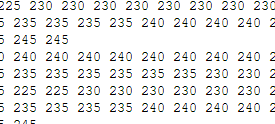
\includegraphics{JuliaPGMScreenshot}
\end{center}

By converting this .pgm file into another format, such as .png, we get a graphic image of our Julia Set.  This can be accomplished a number of ways.  Sage makes it easy with its built in terminal command line at the top of each folder.  Simply type "convert JuliaXXX.pgm JuliaXXX.png" into the terminal, where XXX is the rest of the file name, and you can of course replace .png with the file extension of your choosing.  Sage will then create a new file displaying your Julia Set.

The image is not high resolution due to our creation method, but again it is relatively straightforward and easy to follow which I think makes up for it.  There are many different programs that will create Julia Sets and other fractals, as well as several different iteration methods.  That would be a project by itself and is thus beyond the scope of this project.  Again, if you are interested I encourage you to explore the internet.


%Start of Julia sets
\clearpage
\begin{center}

For these first three images, I used $c$ values that I found online in order to replicate the image and obtain an interesting Julia Set.  That way I knew my code was working.  Plus I would get a variety of well defined Julia Sets, rather than hit-or-miss guessing as you'll see later.

\bigskip
Julia Set with $c = -0.8 + 0.156i$

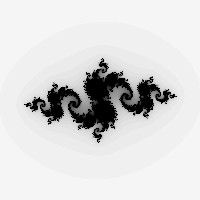
\includegraphics{Julia1}

Julia Set with $c = 0.285 + 0.01i$

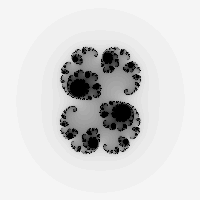
\includegraphics{Julia2}

\clearpage

Julia Set with $c = 0.70176 - 0.3842i$

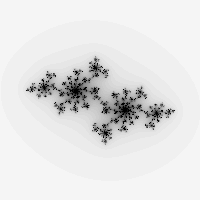
\includegraphics{Julia3}

\bigskip
Starting here, I tested out random $c$ values to see what they would produce.  The results ended up varying greatly.  Some, such as this next image, turned out very cool.

\bigskip
Julia Set with $c = -0.045 + 0.764i$

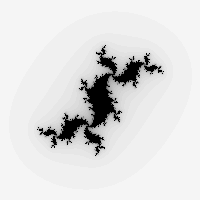
\includegraphics{Julia4}

\clearpage
Others, such as this one, were less interesting.
\bigskip

Julia Set with $c = 0.876 + 0.259i$


\includegraphics{Julia5}

Julia Set with $c = -0.378 - 0.594i$

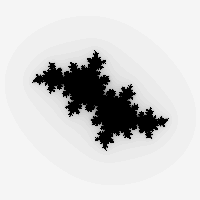
\includegraphics{Julia6}

\clearpage
These two images have an initial $c$ that only varies by $0.05$ in the real component.  As you can see, there is not a tremendous difference.  The top image has darker centers.  However, considering the relatively small change, I think the difference is still significant. 

\bigskip
Julia Set with $c = 0.45 - 0.57i$

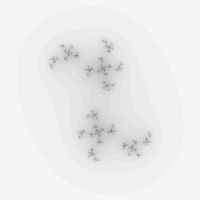
\includegraphics{Julia7}

Julia Set with $c = 0.50 - 0.57i$

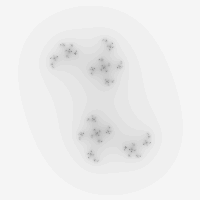
\includegraphics{Julia8}

\clearpage

\end{center}

Fractals have become a large source of inspiration for a variety of artists.  Photographers seek out fractals in nature - like the veins on a leaf, snowflakes, and certain types of brocolli.  Jewelers make a living from creating pendants, bracelets, and rings with fractal images.  3D Printing in particular has opened up a new path for fractals.  I highly suggest taking a few minutes and browsing a site such as Shapeways.com to see what people  are making out of fractals.  In my opinion, it is truly incredible.  

\end{document}
